% Kinematic fitting at ANKE
% Разработанное расширение было использовано авторами для кинематического фита в реакциях $pp \to pp$ и $pp \to pp\pi^0$ на данных, полученных на спектрометре ANKE (Jülich, Germany)~\cite{anke}.
The developed Fumili extension was used by the authors to perform the kinematic fitting of the data obtained at the ANKE spectrometer (Jülich, Germany)~\cite{anke} for the $pp \to pp$ and $pp \to pp\pi^0$ reactions.

% На рисунке \eqref{anke_scheme} можно видеть, что в процессе прохождения протонного пучка через установку часть протонов может отклоняться от направления основного пучка и не фиксироваться установкой, таким образом при анализе данных эксперимента мы можем столкнуться с разницей зафиксированных энергий и количества вещества, вступившего в реакцию с данными, полученными на выходе. Восстановить долю таких ``потерянных'' протонов мы можем, используя инвариант Лоренца $\left|\boldsymbol{P}^{(4)}_\mathrm{beam}+\boldsymbol{P}^{(4)}_\mathrm{targ}-\boldsymbol{P}^{(4)}_p\right|^2 = m_p^2$.

\begin{figure}[htbp]\centering
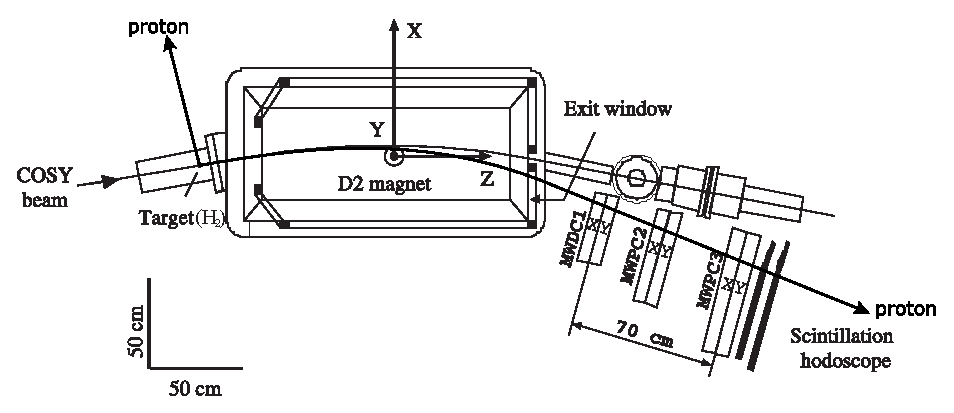
\includegraphics[width=0.8\textwidth]{pics/setup_bw.eps}
\caption{
Scheme of the $pp \to pp$ reaction being registered in the ANKE forward detector. Other ANKE detectors are not shown.
}
\label{anke_scheme}
\end{figure}

\begin{figure}[htbp]\centering
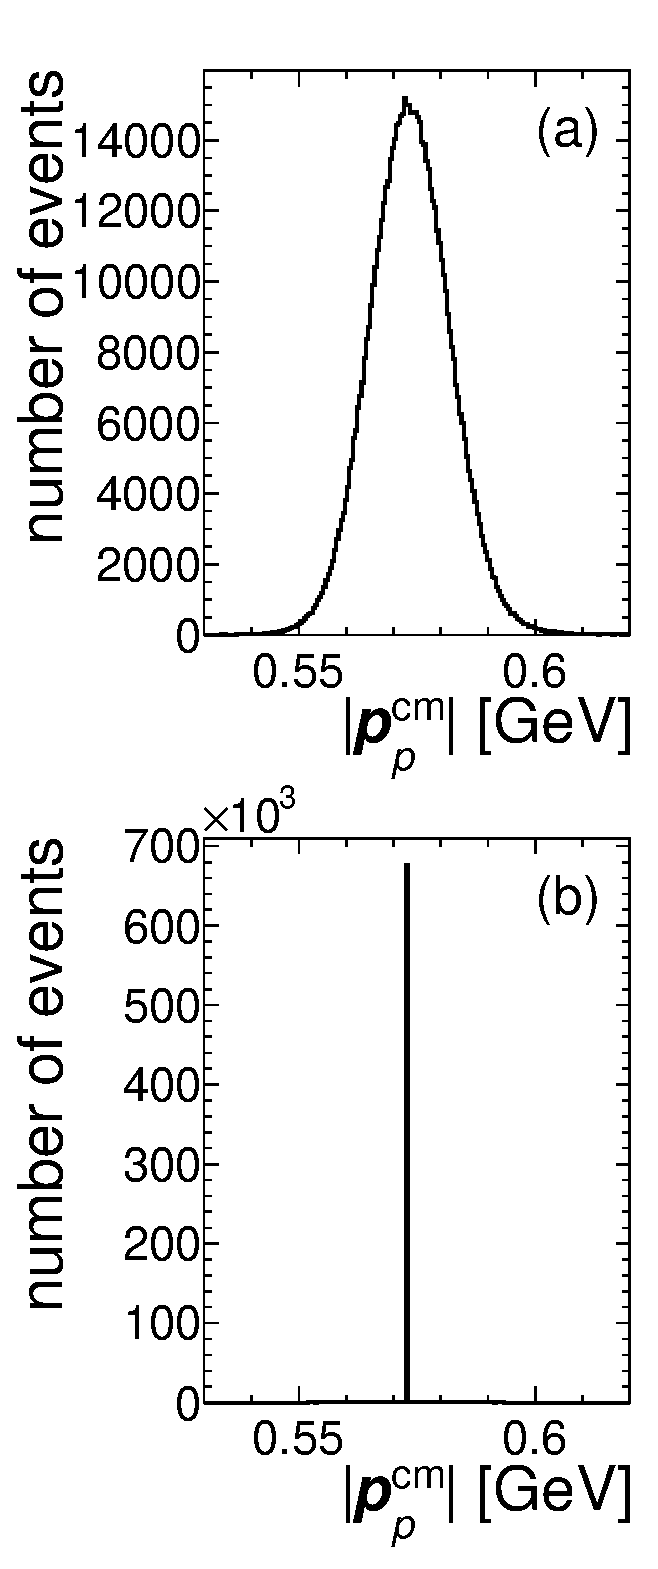
\includegraphics[height=0.3\textheight]{pics/drawMom.eps}
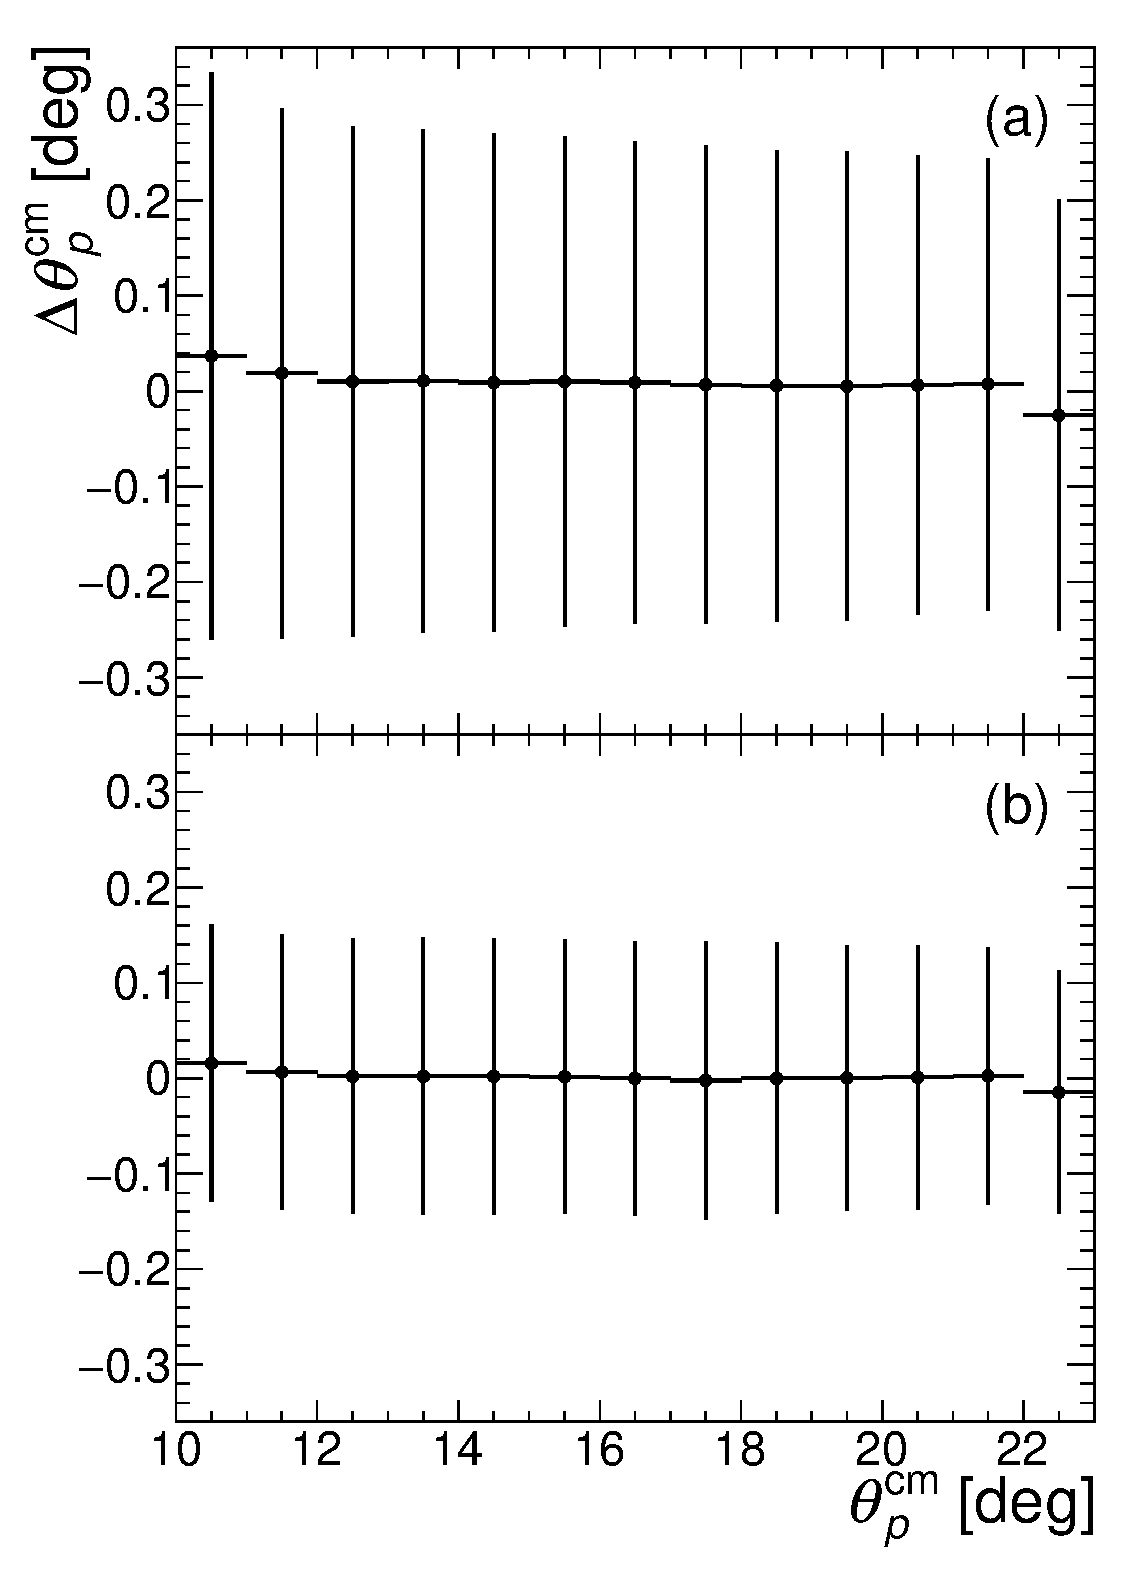
\includegraphics[height=0.3\textheight]{pics/drawTh.eps}
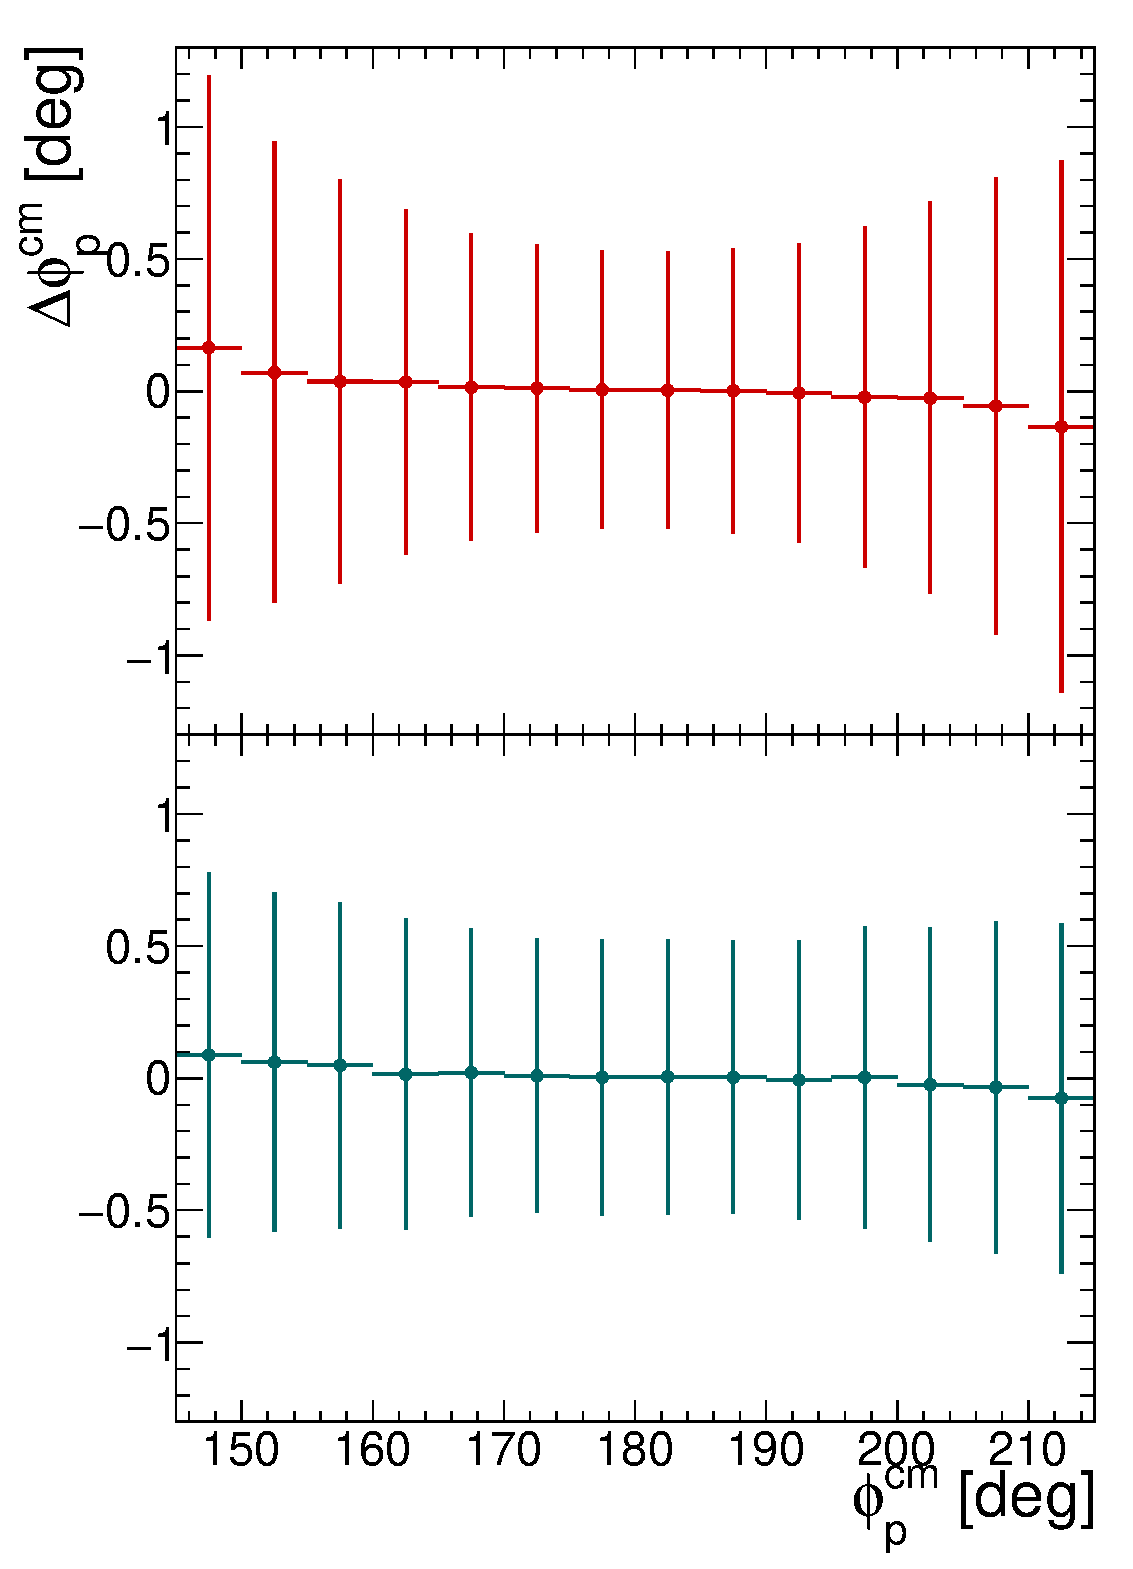
\includegraphics[height=0.3\textheight]{pics/drawPhi.eps}
\caption{
Errors of reconstructed proton momentum in polar coordinates $(|\boldsymbol{p}_p^\mathrm{cm}|, \theta_p^\mathrm{cm}, \phi_p^\mathrm{cm})$ for the $pp \to pp$ reaction at ANKE, simulated for $T_\mathrm{beam} = 700$~MeV either with (a) or without (b) kinematic fitting.
}
\label{anke_errs}
\end{figure}

Let us consider the $pp \to pp$ reaction registered in the forward detector (fig.~\ref{anke_scheme}).
In this case the detector acceptance allows to register only one of the final protons, so we use equation \eqref{cons_miss} for missing mass as a constraint.
Tracking is being done in the forward detector by three multiwire gas chambers, each consisting of several multiwire planes.
A set of signals produced by adjacent wires when a particle passes nearby is called a cluster.
So, an event would contain a set of cluster coordinates $\{c_1, \ldots, c_K\}$ with their errors $\{\delta c_1, \ldots, \delta c_K\}$, and the minimized functional is defined by equation \eqref{track_fit}.
For the study under consideration, the reconstructed coordinates $\hat{c}_k$ are calculated on the basis of the known field map of the analyzing magnet using the Runge–Kutta method, assuming that these particles originated from a point-like source at the center of the target-beam interaction volume.

% Рассмотрим область мишени, изображённую на рис.~\ref{anke_scheme}, где происходит упругое $pp$ взаимодействие и один из протонов регистрируется в координатных камерах Fd.
% Результатом является набор измеренных значений координат кластеров ${C_i:m }$ c ошибками ${\delta C_i}$.

% Истинная координата трека $C_i$ есть функция $C_i = C_i (V, P)$, где вектора $V, P$ содержат координаты вершины и компоненты импульса. Далее делается разумное предположение, что разность $C_i - C_i^m$ распределена по Гауссу с ошибкой ${\delta C_i}$. Функция правдоподобия совокупности измеренных координат
% \begin{equation}
% \label{FPC}
% L_c \approx \prod_i \exp \left(\frac{-1}{2} \left(\frac{C_i - C_i^m}{\delta_{C_i}} \right)^2 \right) \ldotp \Delta C_i
% \end{equation}

% Функция правдоподобия для координат вершины (в предположении, что по каждой координате распределение Гауссово и они независимы; на самом деле функция плотности вероятности распределения по координатам вершины может иметь более сложный вид):
% \begin{equation}
% \label{FPV}
% L_c \approx \prod_i \exp \left(\frac{-1}{2} \left(\frac{V_i - V_i^m}{\delta_{V_i}} \right)^2 \right) \ldotp \Delta V_i
% \end{equation}

% Тогда совместная функция правдоподобия $L_G$ будет иметь вид:
% \begin{equation}
% \label{FPG}
% L_G = L_V \ldotp L_C
% \end{equation}
% Наиболее точная оценка параметров будет получена путём минимизации общей функции правдоподобия $L_G$, однако, если нет информации об $L_V$, оценка параметров производится
% только по $L_C$.

% TODO: Добавить, причем тут Polar CMS coordinates.

% \centering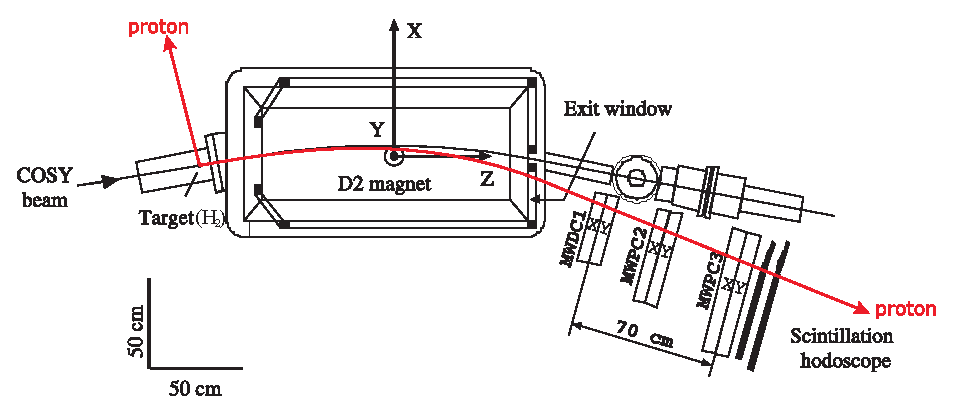
\includegraphics[width=0.8\textwidth]{pics/setup_.eps}

% \large
% \phantom{0}
% 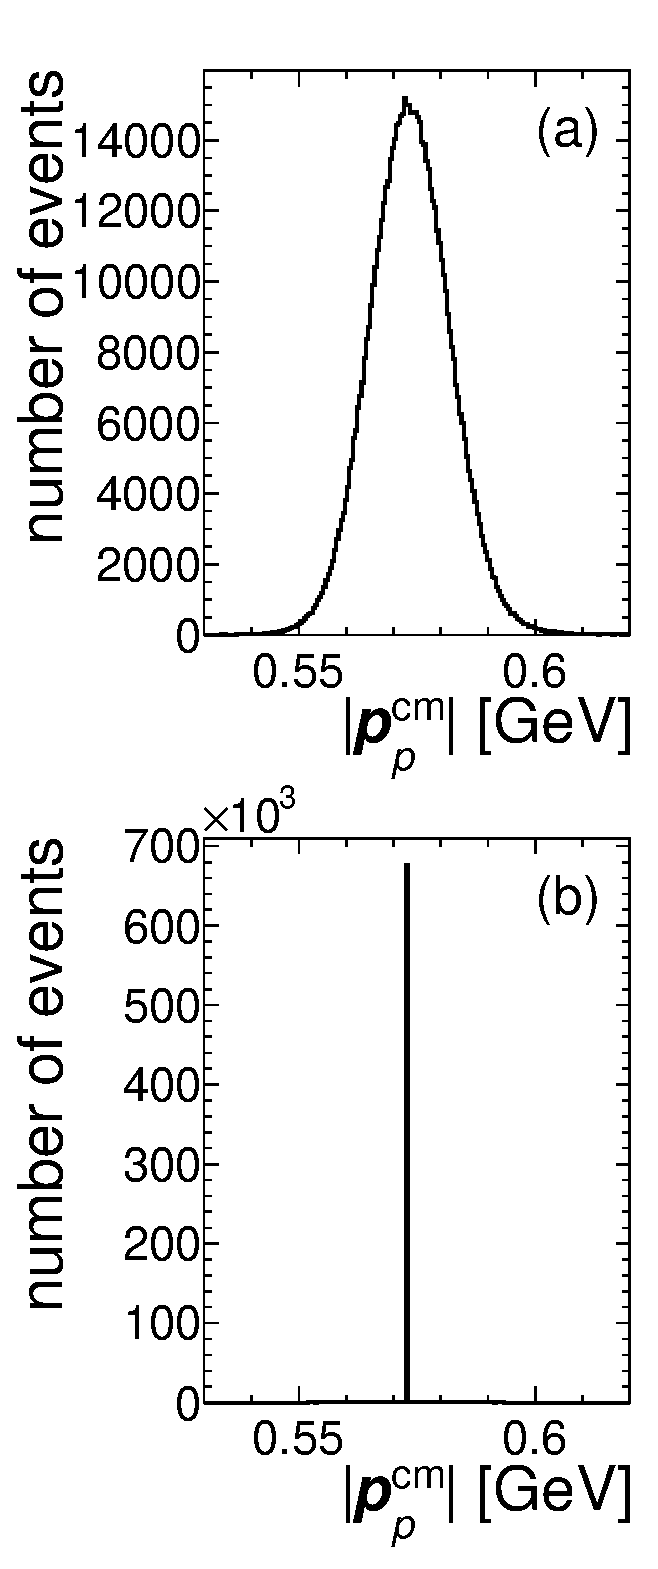
\includegraphics[height=0.7\textheight]{pics/drawMom.eps}
% \hfill
% 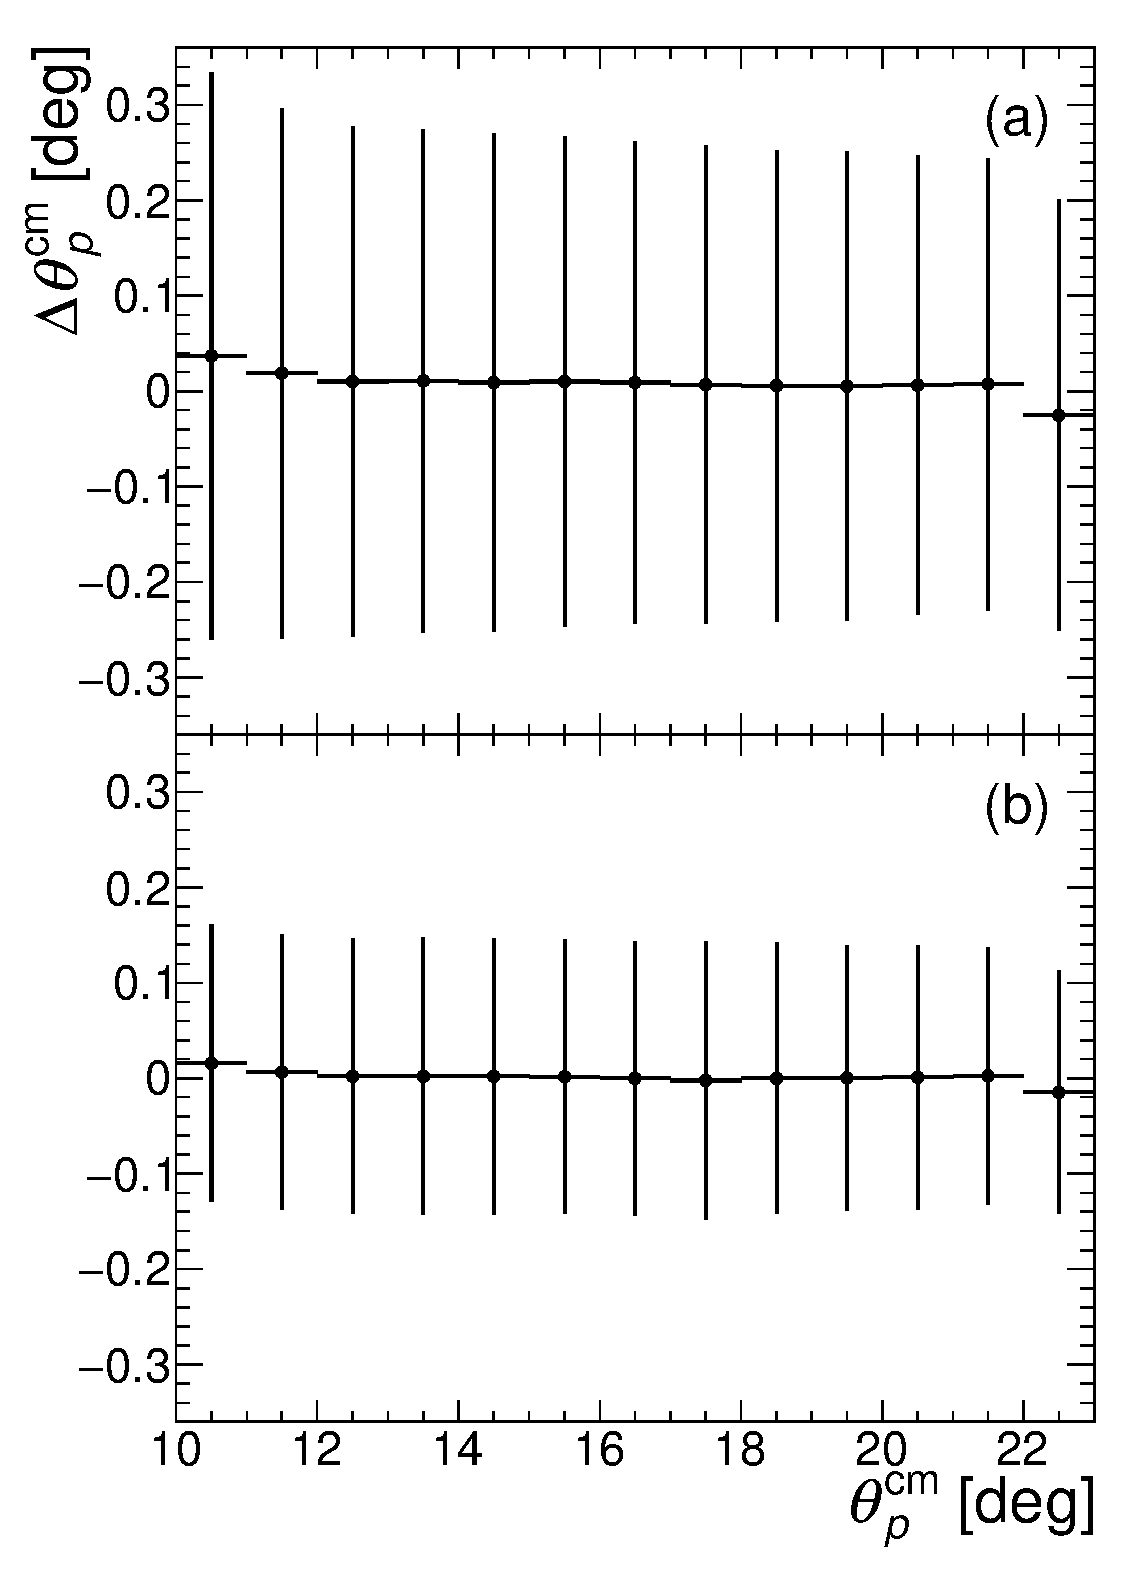
\includegraphics[height=0.7\textheight]{pics/drawTh.eps}
% \hfill
% % \hspace{1em}
% 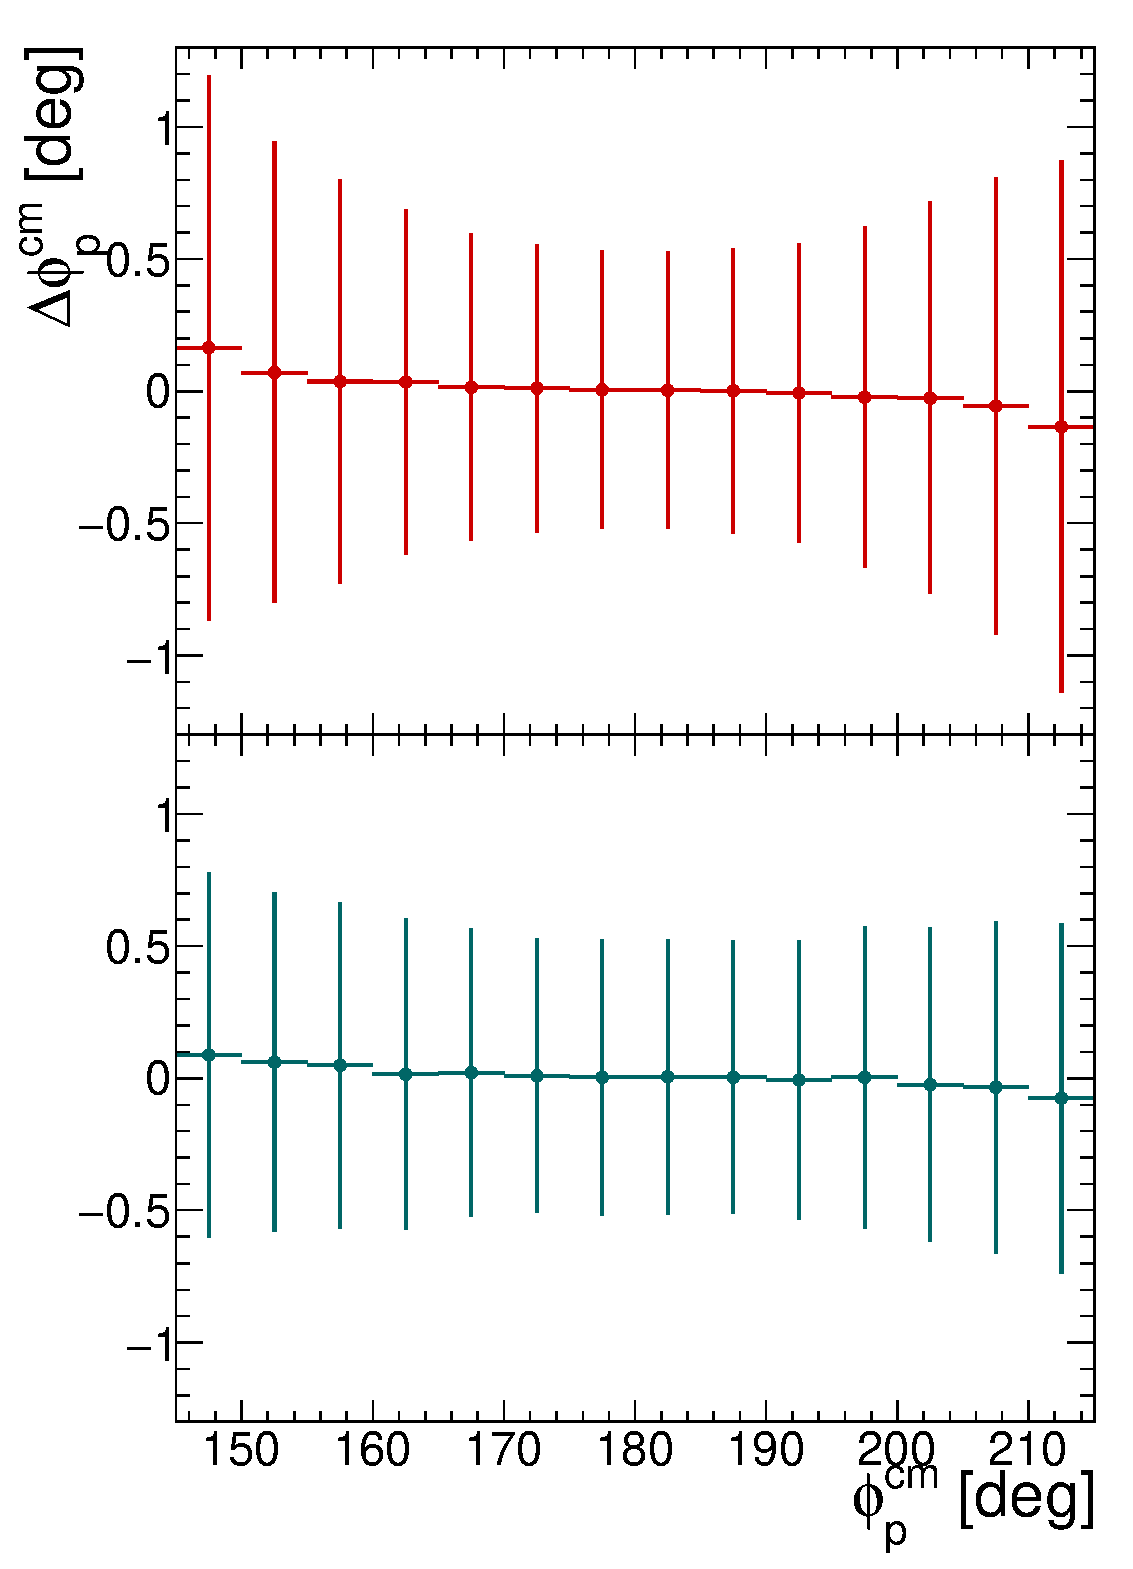
\includegraphics[height=0.7\textheight]{pics/drawPhi.eps}
% \hfill
% \phantom{0}

In order to check the improvement of the momentum precision, about 700\,000 $pp \to pp$ events were simulated and then reconstructed either with or without kinematic constraint \eqref{cons_miss}.
The reconstruction precision for momenta in polar coordinates in center of mass system is shown in fig.~\ref{anke_errs}.
Since $pp \to pp$ is a binary reaction, the condition \eqref{cons_miss} fixes the absolute value of the momentum $|\boldsymbol{p}_p^\mathrm{cm}|$ to the delta function.
Kinematic fitting improves the precision of the polar angle $\theta_p^\mathrm{cm}$ nearly twice.
For the azimuthal angle $\phi_p^\mathrm{cm}$ the improvement not so significant and can be noticed only at the edges of the acceptance.
